\documentclass[a4paper]{article}

% Margins to 2cm
\usepackage[left=2cm,right=2cm,top=3cm,bottom=2cm]{geometry}

% No identation on paragraphs
\usepackage{parskip}

\usepackage[T1]{fontenc}
\usepackage{textcomp}
\usepackage{upquote}
\usepackage{graphicx}

% Allow for code samples and change captions for "Listings" to "Code Snippet"
% \usepackage{minted}
\usepackage{xcolor}
\usepackage{listings} %bera
\definecolor{keywords}{RGB}{0,0,255}
\definecolor{comments}{RGB}{190,190,190}
\lstset{basicstyle=\ttfamily,
language=Python,
  showstringspaces=false,
  commentstyle=\color{red},
  keywordstyle=\color{blue},
  upquote=True
}

% URLS
\usepackage{hyperref}

% Prevent hypenation (not the nicest way to do this)
\hyphenpenalty 1000

% Asterism
\newcommand{\asterism}{\bigskip\par\centerline{*\,*\,*}\medskip\par}%

% Page headers
\usepackage{fancyhdr}

\pagestyle{fancy}
\fancyhf{}
\rhead{Mathematical Algorithms Hack}
\lhead{CS244{\tiny{20}} - CSM01{\tiny{20}} - MA252{\tiny{20}} - MT252{\tiny{20}} - MX352{\tiny{20}}}
\rfoot{\thepage}

% Use a sensible encoding so we don't have fancy quotes
\usepackage[T1]{fontenc}

%%%%%%%%%%%%%%%%%%%%%%%%%%%%%%%%%%%%%%%%%%%%%%%%%%%%%%%
%For hiding and showing solutions:

\usepackage{etoolbox}   % for booleans and much more
\usepackage{verbatim}   % for the comment environment

% setup a new boolean
\newbool{hidesolution}
\setbool{hidesolution}{false}

% new environment
\newenvironment{solution}{}{}

% set conditional behaviour of environment
\ifbool{hidesolution}{\AtBeginEnvironment{solution}{\comment}%
\AtEndEnvironment{solution}{\endcomment}}{}
%%%%%%%%%%%%%%%%%%%%%%%%%%%%%%%%%%%%%%%%%%%%%%%%%%%%%%%


\begin{document}
\begin{center}
    {\huge{Buffon's needles}}\\

\end{center}

\vskip 0.5cm

In 1733 French scientist Buffon was investigating probabilities. He had a large sheet of paper with many equally spaced parallel lines drawn on it. The lines were each a distance of $t$ apart. When he threw needles of a fixed length $l$ down on the paper, some of the needles fell so that they crossed a line, and some fell so that they lay between the lines. 

\begin{figure}[h]
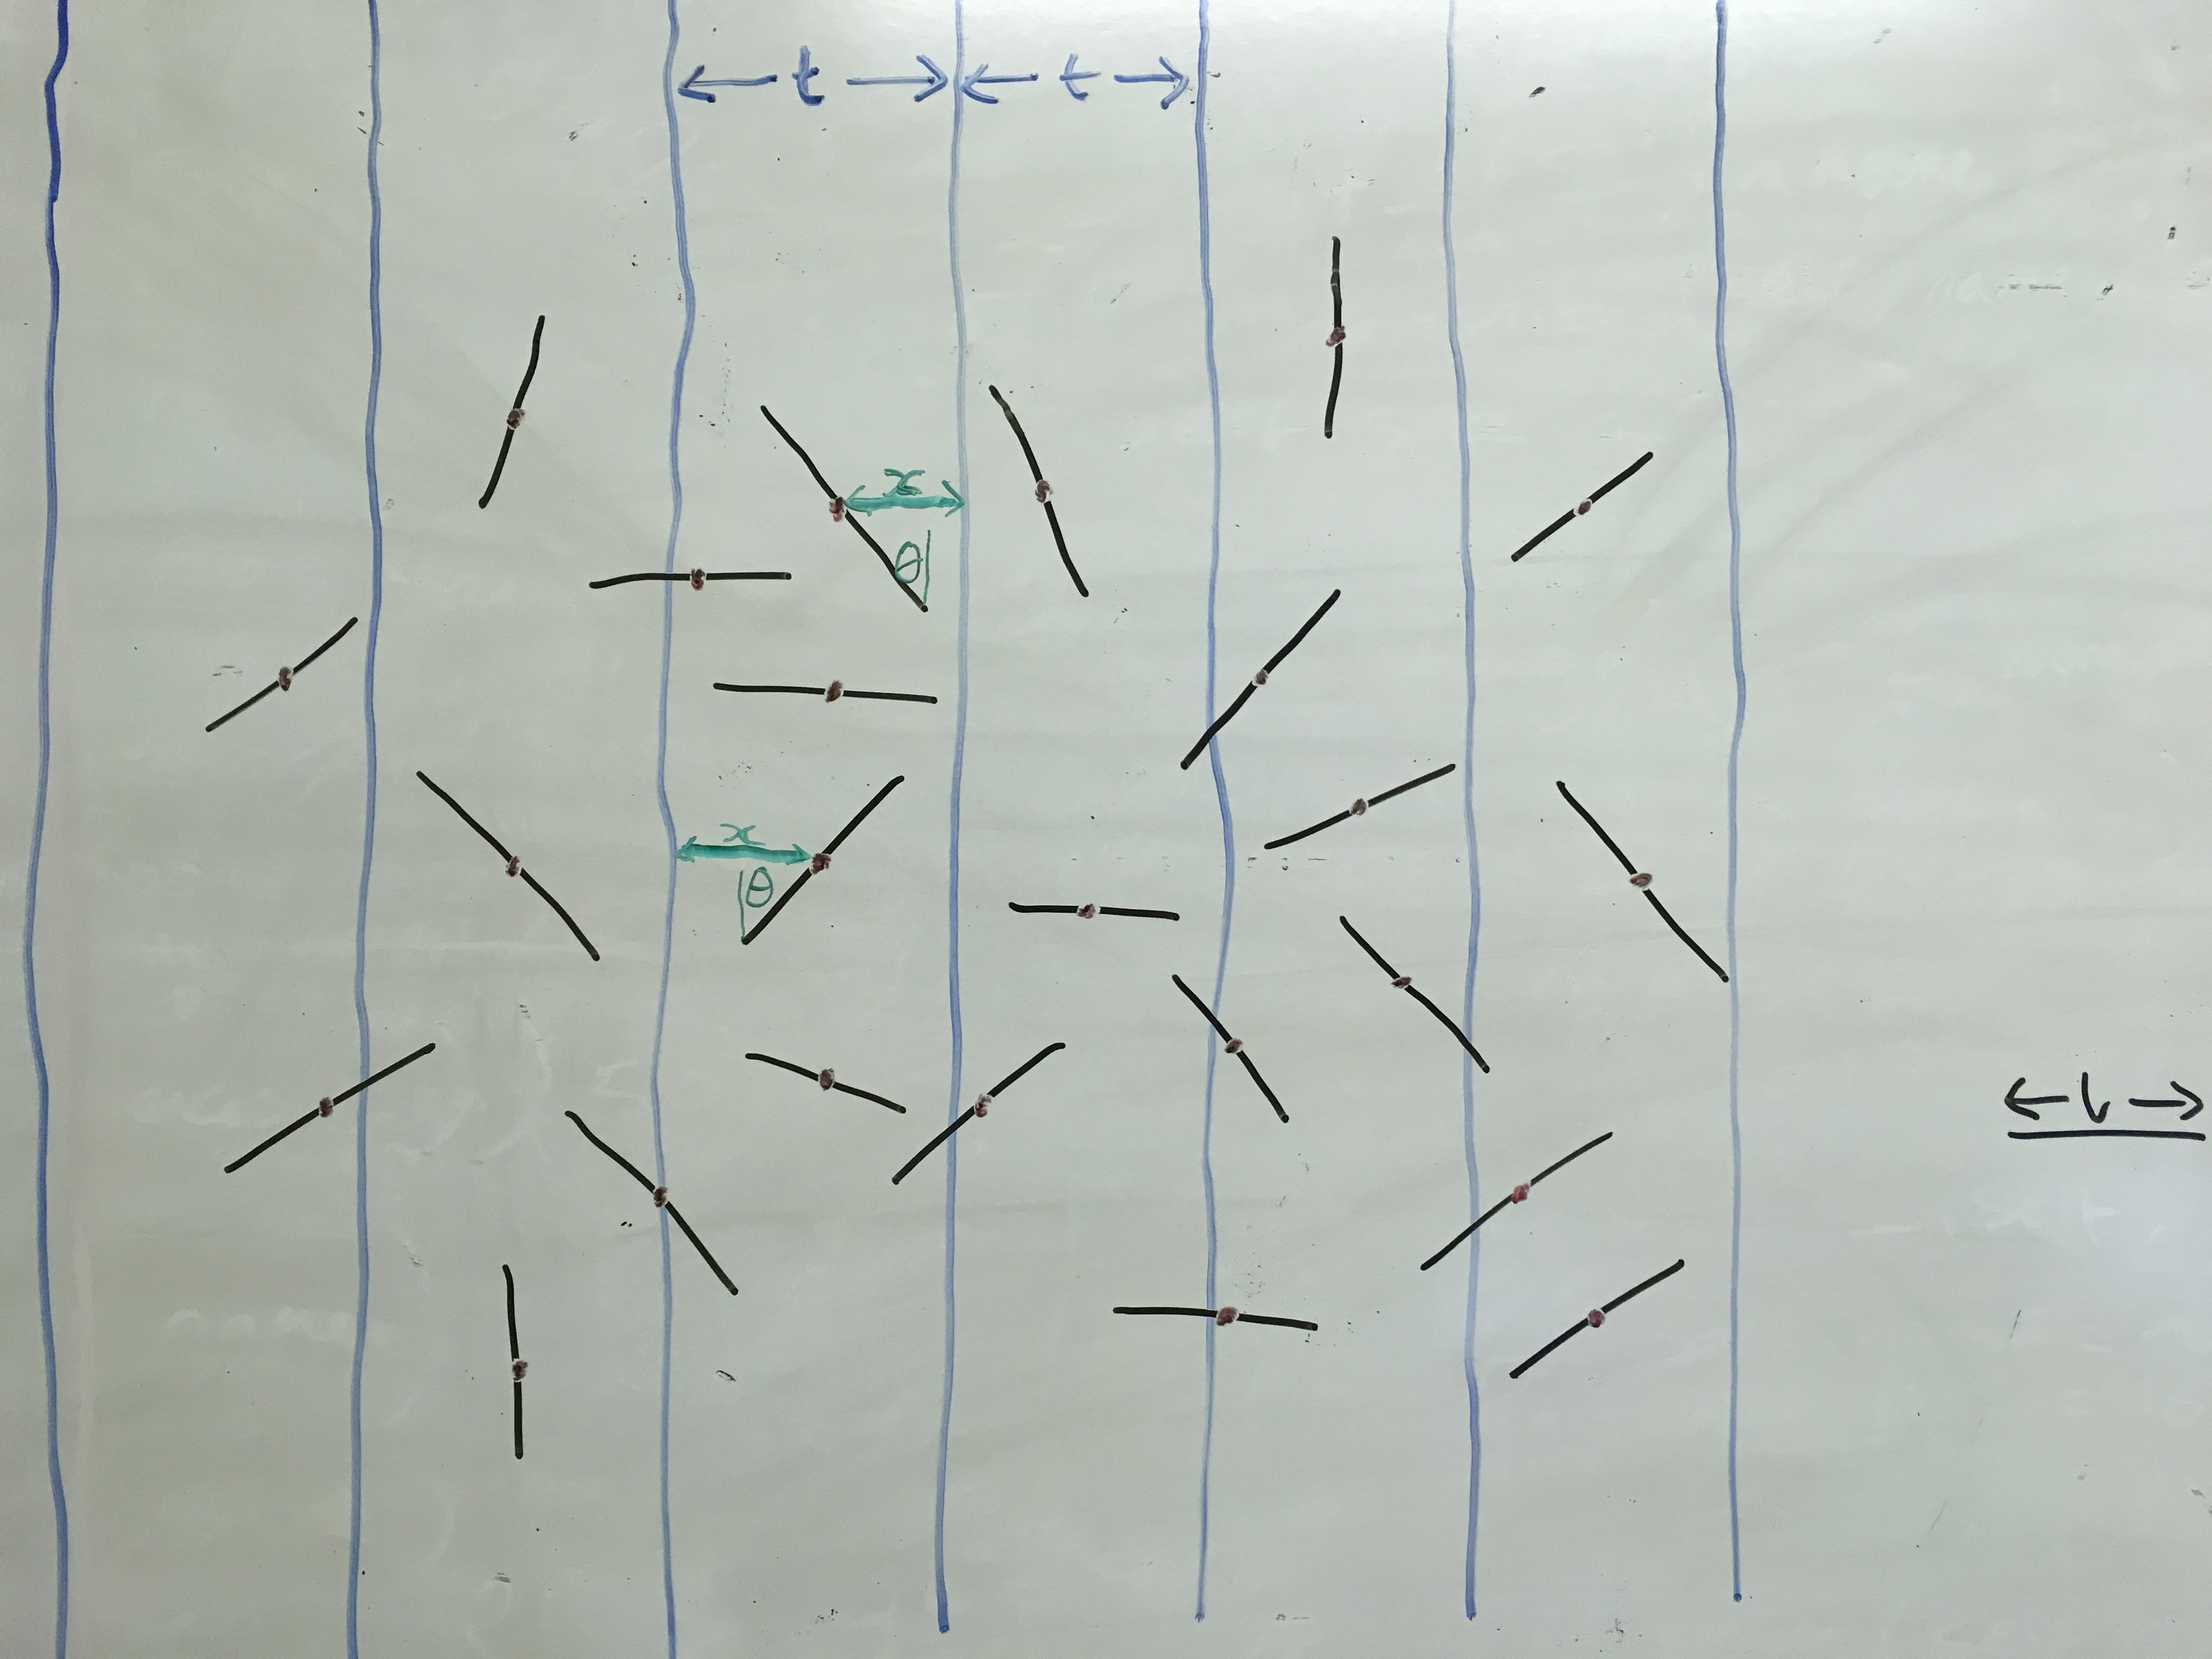
\includegraphics[width=10cm]{IMG_2491.jpg}
\end{figure}

If Buffon throws many needles onto his sheet of paper, he can use their properties to estimate the value of $\pi$.

We want to simulate this experiment, drop lots of needles and therefore find a good estimation of the value of $\pi$.


Each needle has a centre which lies a distance $x$ from the nearest line, and lies at an acute angle $\theta$ to the nearest line.  Two useful facts are as follows:

\begin{enumerate}


\item  A needle crosses a line if 
\[x < \frac{l}{2} \sin(\theta)\]

\item If we generate $n$ random needles, and $h$ of them cross a line then we can find an approximate $\pi$ by using the following:
\[ \pi \approx \frac{2ln}{th} \]
\end{enumerate}


Write code to simulate the dropping of needles and hence estimate the value of $\pi$.

If you want to understand the reasons for these formulae, see: \\
\url{http://mathworld.wolfram.com/BuffonsNeedleProblem.html}

\end{document}